\header{6}
\chapter{Optische Tekens}
\section{Inleiding}
Vanuit het BPR zijn er een aantal regels voor het dragen van optische tekens op je schip. Onder optische tekens vallen zowel navigatieverlichting als dagtekens. In dit hoofdstuk wordt uitgelegd wanneer schepen optische tekens moeten dragen en welke tekens dit zijn. Daarnaast leer je andere schepen aan hun tekens te identificeren.
\newcommand{\RemoveLine}{\vspace*{-2mm}}

\section{Lichten}
In het BPR staat voor verschillende scheepssoorten gespecificeerd welke navigatieverlichting deze moeten dragen. Het BPR verplicht schepen deze tekens te dragen tijdens de nacht (tijd tussen zonsondergang en zonsopgang).

\vspace*{-0.5cm}
\begin{figure}[H]
	\centering
	\begin{minipage}[t]{0.43\textwidth}
		Het BPR kent vier verschillende soorten lichten: toplicht, boordlichten, heklicht en rondom schijnend licht. In figuur \ref{pic:optische_tekens} is een overzicht van de verschillende lichten te zien en welke hoek deze beslaan. In tabel \ref{tab:licht_legenda} zijn de schematische weergaven van deze lichten te zien.
	\end{minipage}
	\hfill
	\begin{minipage}[t]{0.55\textwidth}
		\raisebox{-0.8\height}{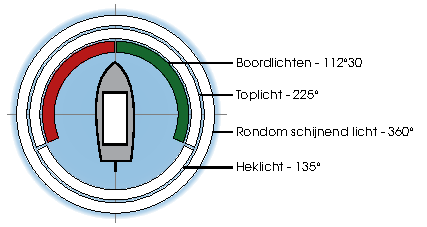
\includegraphics[width=\textwidth]{Hoofdstukken/Optisch/pdf/lichtroos.pdf}}
		\RemoveLine
		\caption{}
		\label{pic:optische_tekens}
	\end{minipage}
\end{figure}

\begin{table}[h]
	\centering
	\caption{Legenda lichten}
	\label{tab:licht_legenda}
	\begin{tabular}{c@{}m{4cm}c@{}m{2.5cm}c@{}m{1.5cm}c@{}m{1.5cm}}
		\raisebox{-0.35\height}{
\includegraphics[height=0.8cm]{Hoofdstukken/Optisch/pdf/rondom_schijnend_licht.pdf}} & \hspace*{1mm}Rondom schijnend licht
		&\raisebox{-0.35\height}{
\includegraphics[height=0.8cm]{Hoofdstukken/Optisch/pdf/boordlicht_bakboord.pdf}}
		\raisebox{-0.35\height}{
\includegraphics[height=0.8cm]{Hoofdstukken/Optisch/pdf/boordlicht_stuurboord.pdf}} & \hspace*{1mm} Boordlichten	
		&\scalebox{-1}[1]{\raisebox{-0.35\height}{
\includegraphics[height=0.8cm]{Hoofdstukken/Optisch/pdf/heklicht.pdf}}} & \hspace*{1mm}Toplicht
		&\raisebox{-0.35\height}{
\includegraphics[height=0.8cm]{Hoofdstukken/Optisch/pdf/heklicht.pdf}} &\hspace*{1mm} Heklicht
	\end{tabular}
\end{table}
%
\section{Dagtekens}
Door het dragen van dagtekens worden omliggende schepen op bepaalde zaken geattendeerd. De voornaamste gebruikte dagtekens zijn:

\begin{itemize}
	\item \textbf{Zwarte kegel:} De zwarte kegel wordt gebruikt om aan te geven dat een zeilschip, naast zijn zeilen, ook zijn motor gebruikt om voort te bewegen.
	\item \textbf{Zwarte bol:} Een zwarte bol geeft aan dat een schip voor anker ligt. 
	\item \textbf{Gele ruit:} Passagiersschepen onder de 20 meter dragen een gele ruit om aan te geven dat zij een passagiersschip zijn (meer dan 12 personen).
	\item \textbf{Sleep cilinder:} Een `sleep'-cilinder (wit-zwart-geel-zwart-wit) toont dat een schip aan het slepen is.
\end{itemize}


\vfil\newpage
\section{Tekens van schepen}
Verschillende schepen zijn verplicht verschillende optische tekens te dragen. Aan de hand van beschrijvingen en figuren worden deze verplichtingen in deze paragraaf toegelicht. 
\subsection{Grote schepen}
% --- Groot motorschip normaal
\begin{figure}[H]
	\centering
	\begin{minipage}[t]{0.75\textwidth}
	%\vspace{-3.5cm}
	\paragraph{Groot motorschip}
	Een alleenvarend groot motorschip voert 's nachts een toplicht (minimaal 4 meter hoog), boordlichten en een heklicht. Deze verlichting is te zien in figuur \ref{pic:optisch:grootmotor}. Het tweede toplicht (op de kajuit) is enkel verplicht als een schip langer is dan 110 meter en moet hoger zijn dat het voorste toplicht.
	\end{minipage}
	\hfill
	\begin{minipage}[t]{0.22\textwidth}
	\raisebox{-0.9\height}{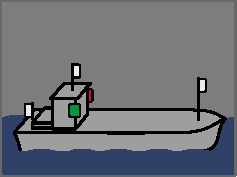
\includegraphics[width=\textwidth]{Hoofdstukken/Optisch/pdf/groot_motorschip.pdf}
	}
	\RemoveLine
	\caption{}
	\label{pic:optisch:grootmotor}
\end{minipage}
\end{figure}
\vspace{-0.6cm}
% --- Groot zeilschip normaal
\begin{figure}[H]
	\centering
	\begin{minipage}[t]{0.75\textwidth}
		\paragraph{Groot zeilschip}
		Figuur \ref{pic:optisch:grootzeil} toont een grootzeilschip bij nacht. Het zeilschip draagt dan boordlichten, een heklicht en twee rondom schijnende lichten in de mast. Het bovenste rondom schijnende licht dient rood te zijn en de onderste groen. 
	\end{minipage}
	\hfill
	\begin{minipage}[t]{0.22\textwidth}
		\raisebox{-0.9\height}{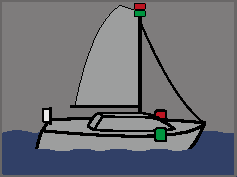
\includegraphics[width=\textwidth]{Hoofdstukken/Optisch/pdf/groot_zeilschip.pdf}}
		\RemoveLine
		\caption{}
		\label{pic:optisch:grootzeil}
	\end{minipage}
\end{figure}
\vspace{-0.6cm}
% --- Groot schip stil
\begin{figure}[H]
	\centering
	\begin{minipage}[t]{0.75\textwidth}
		\paragraph{Stilliggen (oever)}
		Wanneer een groot schip 's nachts aan een oever is afgemeerd, dient deze een wit rondom schijnend licht te dragen. Dit licht moet op minstens 3 meter hoogte geplaatst zijn aan de zijde van het vaarwater. Deze situatie is te zien in figuur \ref{pic:optisch:groot_stil}.
	\end{minipage}
	\hfill
	\begin{minipage}[t]{0.22\textwidth}
		\raisebox{-0.9\height}{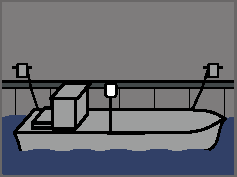
\includegraphics[width=\textwidth]{Hoofdstukken/Optisch/pdf/groot_motorschip_afmeren.pdf}}
		\RemoveLine
		\caption{}
		\label{pic:optisch:groot_stil}
	\end{minipage}
\end{figure}
\vspace{-0.6cm}
% --- Groot schip ankeren
\begin{figure}[H]
	\centering
	\begin{minipage}[t]{0.50\textwidth}
		\paragraph{Ankeren}
		Een groot schip wat 's nachts voor anker ligt moet dit kenbaar maken door het dragen van twee witte rondom schijnende toplichten: een licht voorop het schip en een lager licht achterop het schip. Dit is te zien figuur \ref{pic:optisch:groot_anker}.		
	\end{minipage}
	\hfill
	\begin{minipage}[t]{0.22\textwidth}
		\raisebox{-0.9\height}{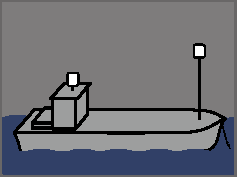
\includegraphics[width=\textwidth]{Hoofdstukken/Optisch/pdf/groot_motorschip_ankeren}}
		\RemoveLine
		\caption{}
		\label{pic:optisch:groot_anker}
	\end{minipage}
	\hfill
	\begin{minipage}[t]{0.22\textwidth}
	\raisebox{-0.9\height}{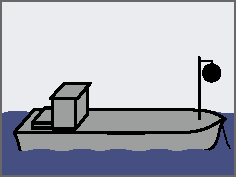
\includegraphics[width=\textwidth]{Hoofdstukken/Optisch/pdf/groot_motorschip_ankeren_dag.pdf}}
	\RemoveLine
	\caption{}
	\label{pic:optisch:groot_anker2}
	\end{minipage}
\end{figure}
\vspace{-0.6cm}
Overdag draagt een groot schip wat geankerd is een zwarte bol. Deze bol dient opgehangen te worden op het voorschip. Deze situatie is te zien in figuur \ref{pic:optisch:groot_anker2}.

% --- Groot schip slepen
\begin{figure}[H]
	\centering
	\begin{minipage}[t]{0.50\textwidth}
		\paragraph{Slepen}
		Wanneer een groot motorschip 's nachts andere schepen sleept dient deze dat kenbaar te maken met de lichten die te zien zijn in figuur \ref{pic:optisch:groot_sleep}: twee toplichten loodrecht boven elkaar, twee boordlichten en een geel heklicht.
	\end{minipage}
	\hfill
	\begin{minipage}[t]{0.22\textwidth}
		\raisebox{-0.9\height}{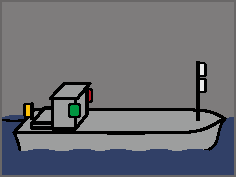
\includegraphics[width=\textwidth]{Hoofdstukken/Optisch/pdf/groot_motorschip_sleep.pdf}}
		\RemoveLine
		\caption{}
		\label{pic:optisch:groot_sleep}
	\end{minipage}
	\hfill
	\begin{minipage}[t]{0.22\textwidth}
		\raisebox{-0.9\height}{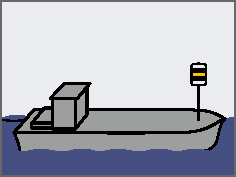
\includegraphics[width=\textwidth]{Hoofdstukken/Optisch/pdf/groot_motorschip_sleep_dag.pdf}}
		\RemoveLine
		\caption{}
		\label{pic:optisch:groot_sleep2}
	\end{minipage}
\end{figure}
\vspace{-0.6cm}
Ieder opvolgend gesleept schip dient een wit rondom schijnend licht te dragen. Het laatste schip dient ook een heklicht te dragen.

Overdag draagt het slepende schip een wit-zwart-geel gekleurde cilinder. Ieder opvolgend schip draagt een gele bol. Het slepende schip is te zien in figuur \ref{pic:optisch:groot_sleep2}.


\subsection{Kleine schepen}

% --- Kleine motorschip
\begin{figure}[H]
	\centering
	\begin{minipage}[t]{0.50\textwidth}
		\paragraph{Klein motorschip}
		's Nachts draagt een klein motorschip navigatieverlichting bestaande uit een toplicht, twee boordlichten en een heklicht. Deze opstelling is te zien in figuur \ref{pic:optisch:klein_motor}. Op deze configuratie zijn echter een aantal variaties toegestaan.		
	\end{minipage}
	\hfill
	\begin{minipage}[t]{0.22\textwidth}
		\raisebox{-0.9\height}{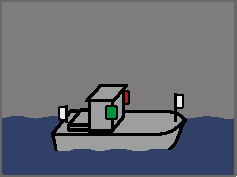
\includegraphics[width=\textwidth]{Hoofdstukken/Optisch/pdf/klein_motorschip.pdf}}
		\RemoveLine
		\caption{}
		\label{pic:optisch:klein_motor}
	\end{minipage}
	\hfill
	\begin{minipage}[t]{0.22\textwidth}
		\raisebox{-0.9\height}{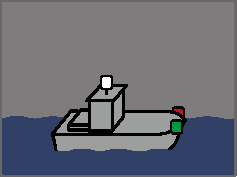
\includegraphics[width=\textwidth]{Hoofdstukken/Optisch/pdf/klein_motorschip_alt.pdf}}
		\RemoveLine
		\caption{}
		\label{pic:optisch:klein_motor2}
	\end{minipage}
\end{figure}
\vspace{-0.6cm}
Zo is het toegestaan de boordlichten in de boeg van het schip te dragen. Ook kan het hek- en toplicht samengevoegd worden in één enkel rondomschijnend toplicht wat minstens een meter hoger is dan de boordlichten. Deze beide variaties zijn in figuur \ref{pic:optisch:klein_motor2} afgebeeld.


% --- Kleine openmotorschip
\begin{figure}[H]
	\centering
	\begin{minipage}[t]{0.75\textwidth}
		\paragraph{Klein open motorschip}
		Een klein \textit{open} motorschip met een lengte van minder dan 7 meter een maximale snelheid van minder dan 13 km per uur hoeft enkel en wit rondom schijnend licht te voeren. Dit is te zien in figuur \ref{pic:optisch:klein_openmotor}.
	\end{minipage}
	\hfill
	\begin{minipage}[t]{0.22\textwidth}
		\raisebox{-0.9\height}{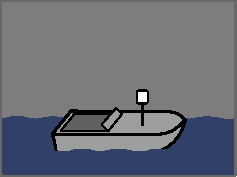
\includegraphics[width=\textwidth]{Hoofdstukken/Optisch/pdf/klein_open_motorschip.pdf}}
		\RemoveLine
		\caption{}
		\label{pic:optisch:klein_openmotor}
	\end{minipage}
\end{figure}


% --- Kleine zeilschip groter dan 7 meter
\begin{figure}[H]
	\centering
	\begin{minipage}[t]{0.50\textwidth}
		\paragraph{Klein zeilschip (>7 meter)}
		Een klein zeilschip draagt 's nachts wanneer deze enkel zeilt drie lichten: twee boordlichten en een heklicht. Deze mogen in twee uitvoeringen gedragen worden. De eerste optie, figuur \ref{pic:optisch:klein_zeil}, heeft boordlichten nabij de boeg van het schip en een heklicht achter op.
	\end{minipage}
	\hfill
	\begin{minipage}[t]{0.22\textwidth}
		\raisebox{-0.9\height}{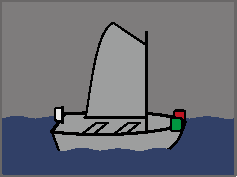
\includegraphics[width=\textwidth]{Hoofdstukken/Optisch/pdf/klein_zeilschip.pdf}}
		\RemoveLine
		\caption{}
		\label{pic:optisch:klein_zeil}
	\end{minipage}
	\hfill
	\begin{minipage}[t]{0.22\textwidth}
		\raisebox{-0.9\height}{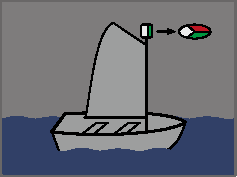
\includegraphics[width=\textwidth]{Hoofdstukken/Optisch/pdf/klein_zeilschip_alt.pdf}}
		\RemoveLine
		\caption{}
		\label{pic:optisch:klein_zeil2}
	\end{minipage}
\end{figure}%
\vspace{-0.6cm}%
De tweede optie verenigt de drie lichten in de mast. In figuur \ref{pic:optisch:klein_zeil2} is dit gecombineerde licht te zien.



% --- Kleine zeilschip met motor
\begin{figure}[H]
	\centering
	\begin{minipage}[t]{0.75\textwidth}
		\paragraph{Klein zeilschip met motor}
		Wanneer een klein zeilschip 's nachts naast zijn zeilen ook een motor gebruikt om zich voort te bewegen, dient deze een toplicht te dragen bij de al voor het zeilschip verplichte lichten. Dit is afgebeeld in figuur \ref{pic:optisch:klein_zeil_motor}. Overdag draagt een zeilschip in deze situatie een kegel. Dit wordt verder toegelicht in paragraaf \ref{par:optisch:overig}
	\end{minipage}
	\hfill
	\begin{minipage}[t]{0.22\textwidth}
		\raisebox{-0.9\height}{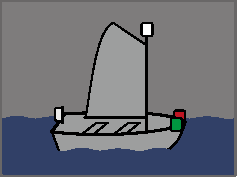
\includegraphics[width=\textwidth]{Hoofdstukken/Optisch/pdf/klein_zeilschip_motor.pdf}}
		\RemoveLine
		\caption{}
		\label{pic:optisch:klein_zeil_motor}
	\end{minipage}	
\end{figure}

% --- Kleine zeilschip >7 meter
\begin{figure}[H]
	\centering
	\begin{minipage}[t]{0.50\textwidth}
		\paragraph{Klein zeilschip (<7 meter) en spier}
		Een zeilschip kleiner dan 7 meter en kleine schepen voortbewogen door spierkracht hoeven 's nachts enkel een rondom schijnend licht te dragen wat van alle zijde goed zichtbaar is. Dit is weergegeven in figuur  \ref{pic:optisch:klein_zeil_klein} en \ref{pic:optisch:klein_spier} .
	\end{minipage}
	\hfill
	\begin{minipage}[t]{0.22\textwidth}
		\raisebox{-0.9\height}{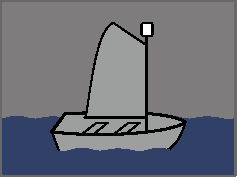
\includegraphics[width=\textwidth]{Hoofdstukken/Optisch/pdf/klein_zeilschip_7m.pdf}}
		\RemoveLine
		\caption{}
		\label{pic:optisch:klein_zeil_klein}
	\end{minipage}
	\hfill
	\begin{minipage}[t]{0.22\textwidth}
		\raisebox{-0.9\height}{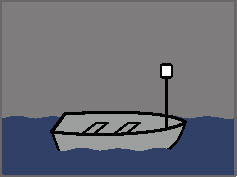
\includegraphics[width=\textwidth]{Hoofdstukken/Optisch/pdf/klein_spier.pdf}}
		\RemoveLine
		\caption{}
		\label{pic:optisch:klein_spier}
	\end{minipage}
\end{figure}%

% --- Kleine slepen
\begin{figure}[H]
	\centering
	\begin{minipage}[t]{0.75\textwidth}
		\paragraph{Klein gesleept schip}
		Wanneer een klein schip 's nachts gesleept wordt door een motorschip, dient deze een wit rondom schijnend licht te dragen. Dit is te zien in figuur \ref{pic:optisch:klein_sleep}. Overdag hoeven kleine schepen die gesleept worden geen speciale tekens te dragen.
	\end{minipage}
	\hfill
	\begin{minipage}[t]{0.22\textwidth}
		\raisebox{-0.9\height}{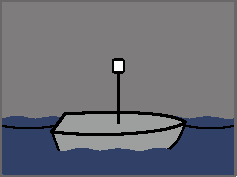
\includegraphics[width=\textwidth]{Hoofdstukken/Optisch/pdf/klein_gesleept.pdf}}
		\RemoveLine
		\caption{}
		\label{pic:optisch:klein_sleep}
	\end{minipage}
\end{figure}

% --- Kleine schip ankeren
\begin{figure}[H]
	\centering
	\begin{minipage}[t]{0.50\textwidth}
		\paragraph{Ankeren}
		's Nachts draagt een klein geankerd schip, net als een groot schip, één wit rondom schijnend toplicht zoals te zien is in figuur \ref{pic:optisch:klein_anker}. Deze verplichting vervalt echter als de omgeving goed verlicht is of het schip op een veilige plaats buiten het vaarwater ligt.
	\end{minipage}
	\hfill
	\begin{minipage}[t]{0.22\textwidth}
		\raisebox{-0.9\height}{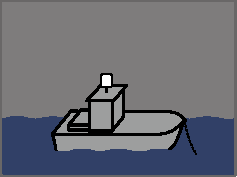
\includegraphics[width=\textwidth]{Hoofdstukken/Optisch/pdf/klein_motorschip_anker.pdf}}
		\RemoveLine
		\caption{}
		\label{pic:optisch:klein_anker}
	\end{minipage}
	\hfill
	\begin{minipage}[t]{0.22\textwidth}
		\raisebox{-0.9\height}{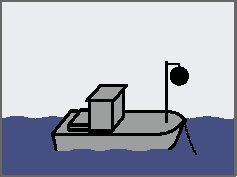
\includegraphics[width=\textwidth]{Hoofdstukken/Optisch/pdf/klein_motorschip_anker_dag.pdf}}
		\RemoveLine
		\caption{}
		\label{pic:optisch:klein_anker2}
	\end{minipage}
\end{figure}%
\vspace{-0.6cm}%
Overdag draag een klein schip, evenals een groot schip, een zwarte bol op het voorschip op een goed zichtbare plaats. Dit is te zien in figuur \ref{pic:optisch:klein_anker2}.


\subsection{Overige tekens}
\label{par:optisch:overig}
% --- Gele ruit
\begin{figure}[H]
	\centering
	\begin{minipage}[t]{0.75\textwidth}
		\paragraph{Passagiers ruit}
		Wanneer een passagiersschip (meer dan 12 personen) een lengte bedraagt van minder dan 20 meter dient deze een gele ruit te dragen op een positie waar deze goed zichtbaar is. De ruit, te zien in figuur \ref{pic:optisch:gele_ruit}, maakt de voorrangspositie van het passagiersschip duidelijk naar de omgeving. 
	\end{minipage}
	\hfill
	\begin{minipage}[t]{0.22\textwidth}
		\raisebox{-0.9\height}{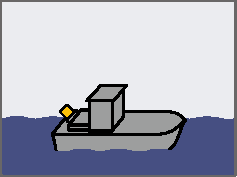
\includegraphics[width=\textwidth]{Hoofdstukken/Optisch/pdf/klein_motorschip_ruit.pdf}}
		\RemoveLine
		\caption{}
		\label{pic:optisch:gele_ruit}
	\end{minipage}
\end{figure}

% --- Zeilschip kegel
\begin{figure}[H]
	\centering
	\begin{minipage}[t]{0.75\textwidth}
		\paragraph{Zeilkegel}
		Wanneer een zeilschip (groot en klein) overdag op zowel een zeil vaart en gebruik maakt van een motor, is het vereist om een zwarte kegel te dragen. Deze kegel dient op een hoge plek geplaatst worden waar deze goed zichtbaar is. Deze kegel is te zien in figuur \ref{pic:optisch:zeilkegel}.
	\end{minipage}
	\hfill
	\begin{minipage}[t]{0.22\textwidth}
		\raisebox{-0.9\height}{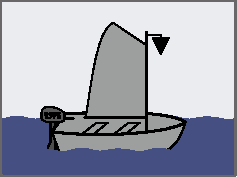
\includegraphics[width=\textwidth]{Hoofdstukken/Optisch/pdf/klein_zeilschip_motor_dag.pdf}}
		\RemoveLine
		\caption{}
		\label{pic:optisch:zeilkegel}
	\end{minipage}
\end{figure}

% --- Schepen in bedrijf
\begin{figure}[H]
	\centering
	\begin{minipage}[t]{0.50\textwidth}
		\paragraph{In bedrijf zijnde werktuigen}
		Schepen die werk uitvoeren op het water (metingen, onderhoud, etc.) kunnen  zowel overdag als 's nachts aangeven welke zijdes langs het schip vrij zijn om te passeren. 
	\end{minipage}
	\hfill
		\begin{minipage}[t]{0.22\textwidth}
		\raisebox{-0.9\height}{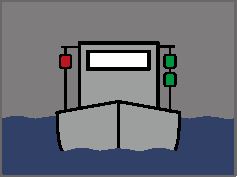
\includegraphics[width=\textwidth]{Hoofdstukken/Optisch/pdf/werktuig.pdf}}
		\RemoveLine
		\caption{}
		\label{pic:optisch:in_bedrijf}
	\end{minipage}
	\hfill
	\begin{minipage}[t]{0.22\textwidth}
		\raisebox{-0.9\height}{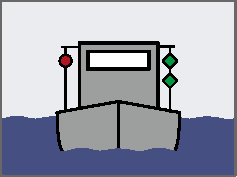
\includegraphics[width=\textwidth]{Hoofdstukken/Optisch/pdf/werktuig_dag.pdf}}
		\RemoveLine
		\caption{}
		\label{pic:optisch:in_bedrijf2}
	\end{minipage}
\end{figure}
\vspace{-0.6cm}%
's Nachts geeft een rood rondom schijnend licht de zijde aan die niet vrij bevaarbaar is. De zijde waar wel langs gevaren mag worden wordt gemarkeerd met twee groene rondom schijnende lichten boven elkaar. In figuur \ref{pic:optisch:in_bedrijf} zijn deze lichten te zien in een vooraanzicht.

Overdag wordt gebruik gemaakt van bollen en ruiten voor het aangeven van vrije en niet-vrije zijdes. De niet vrije zijde is gemarkeerd met een rode bol en de vrije zijde wordt aangegeven met twee groene ruiten boven elkaar. In figuur \ref{pic:optisch:in_bedrijf2} is deze opstelling te zien.

% --- hinder
\begin{figure}[H]
	\centering
	\begin{minipage}[t]{0.75\textwidth}
		\paragraph{Vermijden hinderlijke waterbewegingen}
		Een schip wat werkzaamheden op het water uitvoert kan een teken dragen waarmee verplicht wordt voor omvarenden om hinderlijke waterbewegingen te vermijden. Dit wordt overdag met een rood-wit bord aangegeven en 's nachts met een rood en wit rondom schijnend licht onder elkaar. Zowel de dag als nacht situatie is te zien in figuur  \ref{pic:optisch:hinder}. De borden of lichten gelden alleen aan de zijde van het schip waar deze geplaatst zijn.
	\end{minipage}
	\hfill
	\begin{minipage}[t]{0.22\textwidth}
		\raisebox{-0.9\height}{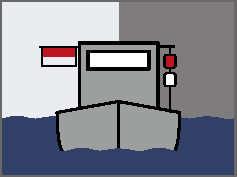
\includegraphics[width=\textwidth]{Hoofdstukken/Optisch/pdf/werktuig_verbod_vaarbeweging.pdf}}
		\RemoveLine
		\caption{}
		\label{pic:optisch:hinder}
	\end{minipage}
\end{figure}

% --- Duiken
\begin{figure}[H]
	\centering
	\begin{minipage}[t]{0.75\textwidth}
		\paragraph{Duiktekens}
		Wanneer er vanaf een schip duiksport wordt uitgeoefend dient dit aangegeven te worden met de internationale seinvlag `A'. Deze vlag is te zien in figuur  \ref{pic:optisch:duik}. In het figuur is deze te zien in combinatie met een ankerbol, omdat dit een veel voorkomende samenstelling is. In de nacht dient de vlag duidelijk verlicht te worden.
	\end{minipage}
	\hfill
	\begin{minipage}[t]{0.22\textwidth}
		\raisebox{-0.9\height}{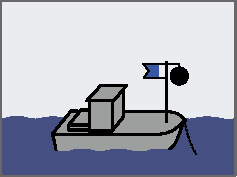
\includegraphics[width=\textwidth]{Hoofdstukken/Optisch/pdf/klein_motorschip_duiker.pdf}}
		\RemoveLine
		\caption{}
		\label{pic:optisch:duik}
	\end{minipage}
\end{figure}

\section{Conclusie}
Na het lezen van dit hoofdstuk heb je kennis van de optische tekens van schepen. Met deze kennis kun je schepen s' nachts aan hun navigatieverlichting herkennen en hierdoor de juiste voorrangsregels toepassen. Ook ken je enkele dagtekens en hun betekenis.